%%%%%%%%%%%%%%%%%%%%%%%%%%%%%%%%%%%%%%%%%%%%%%%%%%%%%%%%%%%%%%%%%%%%%%%%%%%%%%%%
% Preámbulo                                                                    %
%%%%%%%%%%%%%%%%%%%%%%%%%%%%%%%%%%%%%%%%%%%%%%%%%%%%%%%%%%%%%%%%%%%%%%%%%%%%%%%%

\documentclass[11pt,a4paper,titlepage,oneside]{report}

%%% RELACIÓN DE VARIABLES A PERSONALIZAR %%%
%\def\lingua{gal}
\def\lingua{esp} % descomenta esta liña se redactarás a memoria en español
%\def\lingua{eng} % descomenta esta liña se redactarás a memoria en inglés
\def\nome{Brais Barboza Ordóñez}                             % substitúe aquí o teu nome
\def\nomedirectorA{José Antonio Iglesias Guitián}              % substitúe aquí o nome de quen dirixe
\def\nomedirectorB{Francisco Javier Taibo Pena}
\def\nomedirectorC{Emilio José Padrón González}% duplica esta liña máis veces se o precisas, cambiando
                                                     % a letra final (A, B, C, D...): úsanse na portada.tex
\def\titulo{Seguimiento y alineación 3D para la visualización de modelos anatómicos mediante realidad aumentada e impresión 3D} % substitúe aquí o título do teu TFG
%\def\titulacion{gced}                               % descomenta esta liña e comenta a seguinte se es estudante do GCED
\def\titulacion{gei}
%\def\mencion{COMPUTACIÓN}                           % descomenta a mención que che corresponda se es estudante do GEI
%\def\mencion{ENXEÑARÍA DO SOFTWARE}
\def\mencion{ENXEÑARÍA DE COMPUTADORES}
%\def\mencion{SISTEMAS DE INFORMACIÓN}
%\def\mencion{TECNOLOXÍAS DA INFORMACIÓN}

\def\renomearcadros{si} % descomenta esta liña se redactas a memoria en español e prefires que
                         % os "cuadros" e o "índice de cuadros" se renomeen
                         % a "tablas" e "índice de tablas" respectivamente

\usepackage{estilo_tfg}

% Lista de paquetes potencialmente interesantes (uso baixo demanda)

% \usepackage{alltt}       % proporciona o entorno alltt, semellante a verbatim pero que respecta comandos
% \usepackage{enumitem}    % permite personalizar os entornos de lista
% \usepackage{eurofont}    % proporciona o comando \euro
% \usepackage{float}       % permite máis opcións para controlar obxectos flotantes (táboas, figuras)
% \usepackage{hhline}      % permite personalizar as liñas horizontais en arrays e táboas
  \usepackage{longtable}   % permite construir táboas que ocupan máis dunha páxina
% \usepackage{lscape}      % permite colocar partes do documento en orientación apaisada
% \usepackage{moreverb}    % permite personalizar o entorno verbatim
% \usepackage{multirow}    % permite crear celdas que ocupan varias filas da mesma táboa
% \usepackage{pdfpages}    % permite insertar ficheiros en PDF no documento
% \usepackage{rotating}    % permite diferentes tipos de rotacións para figuras e táboas
% \usepackage{subcaption}  % permite a inclusión de varias subfiguras nunha figura
% \usepackage{tabu}        % permite táboas flexibles
% \usepackage{tabularx}    % permite táboas con columnas de anchura determinada

%%%%%%%%%%%%%%%%%%%%%%%%%%%%%%%%%%%%%%%%%%%%%%%%%%%%%%%%%%%%%%%%%%%%%%%%%%%%%%%%
% Corpo                                                                        %
%%%%%%%%%%%%%%%%%%%%%%%%%%%%%%%%%%%%%%%%%%%%%%%%%%%%%%%%%%%%%%%%%%%%%%%%%%%%%%%%

\begin{document}

 %%%%%%%%%%%%%%%%%%%%%%%%%%%%%%%%%%%%%%%%
 % Preliminares do documento            %
 %%%%%%%%%%%%%%%%%%%%%%%%%%%%%%%%%%%%%%%%

 \begin{titlepage}
  
  \hspace*{128pt}
  \textcolor{udcpink}{{\fontencoding{T1}\fontfamily{phv}\selectfont Facultade de Informática}}\\[-32pt]

  \begin{center}
    
\includegraphics[scale=0.3]{imaxes/udc}\\[25pt]

    {\large TRABALLO FIN DE GRAO \\
            GRAO EN ENXEÑARÍA INFORMÁTICA \\
            MENCIÓN EN \mencion } \\[10pt]

    
\includegraphics[scale=0.08]{imaxes/euro_inf_seal_bachelor_light background}\\[25pt]

    \begin{huge}
      \begin{spacing}{1.3}
        \bfseries \titulo
      \end{spacing}
    \end{huge}
  \end{center}
  
  \vfill
  
  \begin{flushright}
    {\large
    \begin{tabular}{ll}
      {\bf Estudiante:} & \nome \\
      {\bf Dirección:}  & \nomedirectorA \\
                        & \nomedirectorB \\
                        & \nomedirectorC\\
    \end{tabular}}
  \end{flushright}
  \rightline{A Coruña, \datasimple.}
\end{titlepage}

 \dedicatoria{A mis padres y mi novia} % escribe neste comando o teu texto de dedicatoria
 \paxinaenbranco
 \begin{agradecementos}
 Dedico este logro académico a aquellos que me han brindado su apoyo incondicional en mi camino. A mis tutores Emilio, Jose y Javi, quienes personificaron la guía necesaria para completar este proyecto con éxito. Gracias por vuestras enseñanzas valiosas y por creer en mí.

A mi familia, especialmente a mis padres, por su amor incondicional y por ser mi constante motivación. Gracias por estar a mi lado en cada decisión y por ser mi fuente de inspiración.

A mis amigos, por su amistad y apoyo en momentos difíciles. Gracias por hacer la vida más alegre e incitarme a alcanzar nuevos horizontes.

Gracias a todos por ayudarme a alcanzar este objetivo. Este trabajo es el resultado de vuestro apoyo y esfuerzo constante, y está dedicado con todo mi agradecimiento y cariño.
 \end{agradecementos}
 %%%%%%%%%%%%%%%%%%%%%%%%%%%%%%%%%%%%%%%%%%%%%%%%%%%%%%%%%%%%%%%%%%%%%%%%%%%%%%%%

\pagestyle{empty}
\begin{abstract}
  La imagen médica se ha beneficiado a lo largo del tiempo de los avances en las técnicas de visualización de contenido con el fin de poder brindar una mejor comprensión de los datos mostrados que se traduzca en una mejor atención médica. Es por ello que en este trabajo se analizan métodos para combinar la imagen médica con la realidad aumentada, otro campo cuyo auge en los últimos años para aplicaciones tanto industriales como de ocio no han pasado desapercibidas. Se lleva a cabo un análisis completo para proporcionar una solución funcional, desde la segmentación de los modelos desde una Tomografía Computerizada (TC), el desarrollo de un marcador para el seguimiento y la alineación en 3D hasta la implementación de una solución para llevarlo a cabo. Con el objetivo de servir como discusión de futuros desarrollos, se concibe teniendo como piedra angular su libre disposición y el software libre como alternativa a métodos existentes tras licencias restrictivas.

  \vspace*{25pt}
  \begin{segundoresumo}
    Medical imaging has benefited over time from advances in content visualization techniques in order to provide a better understanding of the displayed data, leading to improved healthcare. Therefore, this project examines methods for combining medical imaging with augmented reality, another field whose recent rise for both industrial and recreational applications has not gone unnoticed. A comprehensive analysis is carried out to provide a functional solution, including model segmentation from a computerized tomography (CT) scan, marker development for tracking and 3D alignment, and the implementation of a solution to execute the process. In order to serve as a discussion of future developments, this work is conceived with the cornerstone of open availability and open-source software as an alternative to existing methods with restrictive licenses.
  \end{segundoresumo}
  \vspace*{25pt}
  \begin{multicols}{2}
\begin{description}
\item [\palabraschaveprincipal:] \mbox{} \\[-20pt]
  \begin{itemize}
    \item Realidad aumentada
    \item Impresion 3D
    \item Imagen médica
  \end{itemize}
\end{description}
\begin{description}
\item [\palabraschavesecundaria:] \mbox{} \\[-20pt]
  \begin{itemize}
    \item Augmented reality
    \item 3D Printing
    \item Medical imaging
  \end{itemize}
\end{description}
\end{multicols}

\end{abstract}
% \textbf{Herramientas y tecnologías empleadas:}
% \begin{itemize}
%     \item Hardware:
%     \begin{itemize}
%         \item Desarrollo: Portátil Intel core i7 @2.5GHz, 16 GB RAM, Nvidia Geforce 1050.
%         \item Pruebas: PC 12th Gen Intel(R) Core(TM) i9-12900KF   3.20 GHz, 64,0 GB RAM, Nvidia RTX 3090.
%     \end{itemize}
%     \item Software:
%         \begin{itemize}
%             \item S.O: Windows 11.
%             \item Lenguajes: C++.
%             \item Librerías: OpenCV, OpenXR.
%             \item Compilación: Cmake
%             \item Otras Herramientas: ViveSR Works
%         \end{itemize}
% \end{itemize}
\pagestyle{fancy}

%%%%%%%%%%%%%%%%%%%%%%%%%%%%%%%%%%%%%%%%%%%%%%%%%%%%%%%%%%%%%%%%%%%%%%%%%%%%%%%%


 \pagenumbering{roman}
 \setcounter{page}{1}
 \bstctlcite{IEEEexample:BSTcontrol}

 \tableofcontents
 \listoffigures
 \listoftables
 \clearpage
 
 \pagenumbering{arabic}
 \setcounter{page}{1}

 %%%%%%%%%%%%%%%%%%%%%%%%%%%%%%%%%%%%%%%%
 % Capítulos                            %
 %%%%%%%%%%%%%%%%%%%%%%%%%%%%%%%%%%%%%%%%

 \chapter{Introducción}
\label{chap:introducion}

%% Borra esta anotación que che fago no teu seguinte commit
{\color{red} Emilio:}
{\color{gray} Movínche este parágrafo fóra da Motivación, para que o
  modifiques/mellores e sirva como entradiña para este capítulo de
  Introdución, de forma que na motivación presentes xa directamente o
  que nos propoñemos, e antes (aquí) introduzas o tema a tratar con un
  ou dos parágrafos, como este que tes, pero que hai que pulir un
  pouco:
  \begin{itemize}
  \item Tenta usar unha linguaxe o máis natural posible, que non soe
    forzada. Ademais, as frases, canto máis simples, mellor.
  \item Presenta e enlaza ben as ideas: no que dis, engade unha idea
    do que é a imaxe médica (como fas no resumo) e logo enlazas co
    tema da AR como un bo complemento nese eido, un pouco como o que
    temos no primeiro parágrafo do anteproxecto.
  \item Tenta fuxir dunha linguaxe excesivamente comercial,
    minimizando adxectivos que soan a `ventas', como aquí o de
    ``respuesta sólida''.
  \item Fíxate no {\tt .tex} en como poño as aspas/comillas, tanto as
    simples como as dobres, que é o xeito normal de facelo en \LaTeX.
  \end{itemize}
}
%% Borra o anterior ata aquí

\lettrine{D}{ebido} a los continuos avances en la tomografía computerizada, y en la medicina misma, las técnicas para reproducir estos conjuntos de datos, se han vuelto más y más importantes en los últimos 30 años como indica \cite{Botha2014}. En procura de estos nuevos métodos, se han establecido numerosos precedentes de la aplicación de la realidad aumentada en la medicina \cite{Sielhorst2008} ya que es posible su implementación en gran cantidad de tareas del sistema sanitario. Desde divulgación científica hasta cirugía guiada por imagen, la realidad extendida \footnote{Compendio de realidad virtual, realidad aumentada y realidad mixta.} se presenta como una respuesta sólida ante los problemas que acarrea la representación de información del ámbito médico.


\subsection{Motivación}

%% Borra esta anotación que che fago no teu seguinte commit
{\color{red} Emilio:}
{\color{gray} Escribe como motivación un texto parecido ao que temos
  no anteproxecto en 'breve descrición', un pouco máis elaborado (pero
  tampouco moito), e descartando o primeiro parágrafo que quizais
  encaixaría máis para o que comento arriba, para presentar o tema
  antes de comezar coa motivación. Non pasa nada se queda un chisco
  redundante cos obxectivos, que veñen despois. Aquí a idea é que
  quede máis «redactado» que é o que queremos facer, e tamén incluíndo
  o por que o queremos facer, mentres que os obxectivos son máis
  concretos e pormenorizados.
}
%% Borra o anterior ata aquí

\subsection{Objetivos}
Los objetivos principales de este proyecto son:
\begin{itemize}
    \item Analizar y diseñar marcas o guías a partir de imágenes capturadas mediante \acrfull{tc} para su impresión 3D, de forma que faciliten posteriormente el registro y seguimiento en 3D de los datos contenidos en la \acrshort{tc}.

%% Borra esta anotación que che fago no teu seguinte commit
{\color{red} Emilio:}
{\color{gray} A min quédame confuso este primeiro obxectivo (si, xa
  sei que o temos así literalmente no anteproxecto\ldots).  Eu poría
  primeiro quizais primeiro un obxectivo de extraer un modelo 3D a
  partir dun TC, e logo o de analizar e deseñar marcas ou guías para
  ser impresas tamén en 3D e facilitar o rexistro e seguimento e
  blabla.
}
%% Borra o anterior ata aquí

    \item Hacer detección, seguimiento y alineamiento 3D de la pieza impresa o guía en el flujo de vídeo capturado por un sistema de realidad aumentada, como puede ser un \acrshort{hmd} que incorpore cámaras de vídeo.
    \item Integrar elementos sintéticos en la imagen real de la visualización 3D.
    \item El objetivo final es disponer de un software capaz de resolver el problema del seguimiento y la estimación de pose en 3D y que pueda ser fácilmente integrable en un sistema de realidad Extendida completo
\end{itemize}

\subsection{Estructura de la memoria}

TODO

\subsection{Trabajo Previo}

%% Borra esta anotación que che fago no teu seguinte commit
{\color{red} Emilio:}
{\color{gray} Todo isto iría ao capítulo de Estado del Arte, non?
  Este capítulo 1, que habitualmente é un dos máis curtos da memoria,
  concluiría coa descrición da estrutura da memoria, que xa faremos
  cando teñamos máis ou menos todo escrito.
}
%% Borra o anterior ata aquí


\subsubsection{Visualización}
Los componentes artificiales que deseamos incluir en las imágenes del mundo real proceden del framework desarrollado por \citeauthor{Kroes2012} que aplica técnicas de \acrfull{mcrt} sobre \acrfull{dvr}.
\paragraph{}
El termino \acrshort{dvr} se utiliza para referirse a las técnicas que producen una imagen directamente a partir de datos de un volumen, sin realizar pasos intermedios. Para que esto sea posible es necesario implementar modelos físicos que indiquen cómo se genera, refleja, dispersa o oculta la luz \cite{Max1995}. Estos modelos con el paso del tiempo han evolucionado en modelos más y más complejos que han probado ser beneficiosos para la visualización científica de modelos 3D \cite{Daz2015}, \cite{Englund2016}, \cite{Lindemann2011} .

\paragraph{}
La implementación de estos modelos conlleva altos tiempos de renderizado, o en su defecto, un equipo increíblemente costoso para poder obtener una experiencia interactiva \cite{IglesiasGuitian2022}. Para enfrentar esta casuística,  \citeauthor{IglesiasGuitian2022} implementan un algoritmo de reducción de ruido basado en \acrfull{rls} que permite una experiencia interactiva en tiempo real, sobre \acrshort{gpu}s comerciales. Este proyecto se fundamenta en \cite{IglesiasGuitian2022} para el renderizado de las imágenes que posteriormente se apliquen en realidad aumentada sobre las imágenes reales.

\subsubsection{Realidad Extendida}
En 1994 \citeauthor{Milgram1994ATO} describe la realidad extendida como un subconjunto de tecnologías de la \acrfull{vr} que incorporan la mezcla entre el mundo real y el mundo virtual. 
Dado que existen tantas connotaciones y matices de realidad, \citeauthor{Milgram1994ATO} acuña el término de \textbf{\textit{virtuality continuum}}.
\paragraph{}
Este concepto de virtuality continuum \ref{fig:vc}, se caracteriza por comprender desde un usuario completamente inmerso en un mundo sintético que se comporta con algunas de las propiedades físicas del mundo real (incluso desafiando conceptos como la gravedad el tiempo o el espacio), hasta un usuario experimentando el mundo real con elementos virtuales añadidos o superpuestos.
Existen 4 conceptos bien diferenciados dentro del virtuality continuum:
\begin{itemize}
    \item Entorno Real (Real Enviroment): Consiste únicamente en objetos reales, situado al extremo izquierdo de \ref{fig:vc}.
    \item Realidad Aumentda(Augmented Reality): Mundo real aumentado o compuesto por elementos digitales.
    \item Virtualidad Aumentada(Augmented Virtuality): Mundo digital aumentado por objetos reales o fisicos.
    \item (Virtual Enviroment): Entorno puramente virtual.
\end{itemize}

\begin{figure}[hp!]
  \centering
  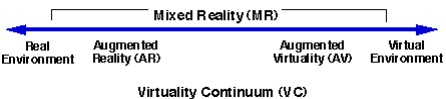
\includegraphics[width=0.75\textwidth]{imaxes/virtuality_continuum.png}
  \caption{Representacion simplificada de un virtuality continuum.}
  \label{fig:vc}
\end{figure}



Posteriormente \citeauthor{Azuma1997} definía la realidad aumentada como una variación de la realidad virtual, en la cual el usuario es capaz de ver el mundo real, con objetos virtuales superpuestos, o compuestos por el mundo real. La posibilidad de crear objetos y prototipos de forma rápida, sobre los cuales poder iterar y componer imágenes virtuales, demuestra el potencial de estas tecnologías trabajando a la par.
\paragraph{}

Para llevar a cabo el proyecto existen varias aproximaciones en el estado del arte \cite{Venkatesan2021}, así que se seleccionaron aquellas que más se ajustaban al proyecto.

--Discutir Aproximaciones--

Uno de los objetivos principales es el seguimiento de piezas extraídas de un \acrshort{tc} y diseñar marcadores que facilitasen el registro de las mismas, por lo que se optó por un seguimiento basado en marcadores. No obstante, en lo que a la visualización se refiere, es necesario un equipo con gran potencia computacional, o en su defecto, un visor que permita la reproducción de vídeo renderizado por un tercer equipo. Dadas estas restricciones se decidió por utilizar un \acrfull{hmd} HTC VIVE PRO. Utilizando \ref{fig:vrAproximations} como referencia, el sistema implementado se compondría de un seguimiento basado en marcadores (E) visualizando estos marcadores en realidad aumentada (B).


Para este proyecto se escogieron las tecnologías E y G que se observan en \ref{fig:vrAproximations}

\begin{figure}[hp!]
  \centering
  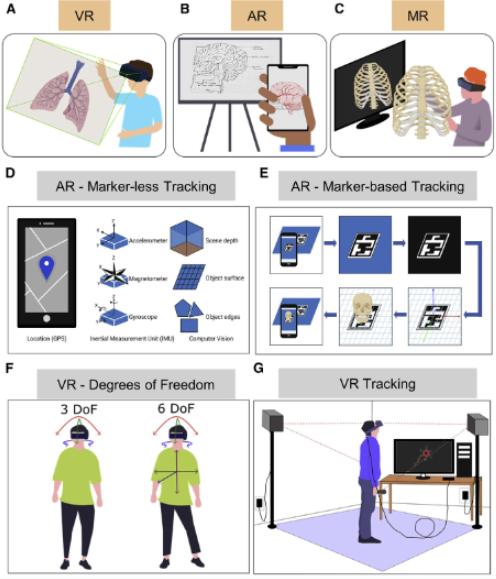
\includegraphics[width=0.75\textwidth]{imaxes/aproxVR.png}
  \caption{Aproximaciones a la realidad extendida para aplicaciones biomédicas.}
  \label{fig:vrAproximations}
\end{figure}


\subsubsection{Impresión 3D}
La impresión 3D o fabricación aditiva es un proceso para manufacturar objetos de cualquier forma o tamaño a partir de un modelo 3D o otro tipo de fuente electrónica a partir de procesos aditivos en los que sucesivas capas de material se depositan bajo control de un ordenador \cite{yan_dong_su_han_song_wei_shi_2018}.
Desde 1984 \cite{ChanaRodrguez2016} hasta la actualidad, la impresión 3D ha afrontado una revolución que se fundamenta en pilares sólidos como el abaratamiento de los costes de producción de impresoras 3D, la mejora de su precisión y velocidad, el software libre, la comercialización de los productos a usuarios finales , documentación, formación extensa corroborada y creada por terceros que facilita y realimenta el desarrollo de nuevos proyectos.
Producto de esto, ha sido la implementación de esta tecnología en el ámbito sanitario, tanto para la producción de herramientas especializadas \cite{ChanaRodrguez2016} como para el diseño y la implantación de prótesis personalizadas para cada paciente \cite{Gonzalez_Alvarez_2021}.




 \chapter{Fundamentos Teóricos}
\label{chap:ft}
En este capítulo se repasan los principios básicos sobre los que se establece este trabajo.
\section{Tomografía Computerizada}
\lettrine{U}{na} \acrfull{tc} en esencia, es una máquina de rayos X en la cual se ha sustituido la placa por una serie de detectores\cite{muniz2006introduccion}. El tubo de Rx emite un haz colimado que atraviesa al paciente. De dicho tubo emerge el haz atenuado remanente que es recibido por el detector mientras efectúa un movimiento circular y avanzando lentamente hasta cubrir el área deseada como se puede ver en \ref{fig:tac}.
\begin{figure}%
    \centering
    \subfloat[\centering Orientación del tubo de rayos X respecto al eje corporal.]{{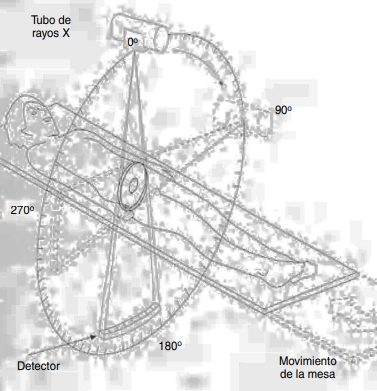
\includegraphics[width=5cm]{imaxes/tac.png} }}%
    \qquad
    \subfloat[\centering Tomografía axial computerizada convencional.]{{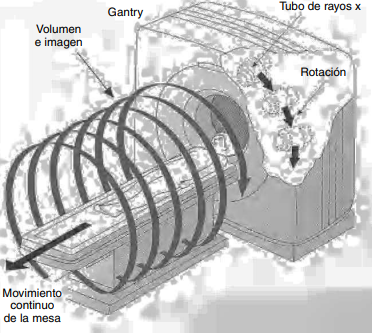
\includegraphics[width=5cm]{imaxes/tacm.png} }}%
    \caption{Representación del funcionamiento de un \acrshort{tc}}%
    \label{fig:tac}%
\end{figure}

\subsection{Teorema de Radon}
El Teorema de Radon, propuesto por el matemático austríaco Johann Radon en 1917, es un resultado fundamental en la teoría de la tomografía computerizada. Este teorema establece que es posible reconstruir una función bidimensional a partir de sus proyecciones a lo largo de diferentes ángulos. En el contexto de la tomografía computerizada, las proyecciones se obtienen mediante la medición de la atenuación de la radiación a medida que atraviesa el objeto en estudio. El Teorema de Radon proporciona la base matemática para la reconstrucción de imágenes en la tomografía computerizada y ha llevado al desarrollo de diversos algoritmos de reconstrucción.

\subsection{Algoritmos de reconstrucción de imágenes}
Los algoritmos de reconstrucción de imágenes son métodos computacionales utilizados para reconstruir imágenes bidimensionales o tridimensionales a partir de proyecciones adquiridas en la tomografía computerizada. Estos algoritmos se basan en el Teorema de Radon y pueden clasificarse en dos categorías principales: métodos analíticos \cite{kontaxakis2002reconstruccion} y métodos iterativos \cite{Willemink2013}.

1. Métodos analíticos: Estos algoritmos, como la retroproyección filtrada (FBP, por sus siglas en inglés), procesan las proyecciones de manera directa para obtener la imagen reconstruida. La FBP es el algoritmo más utilizado en la práctica clínica debido a su rapidez y eficiencia.

2. Métodos iterativos: Estos algoritmos, como el de máxima verosimilitud de la expectativa-maximización (MLEM) y el de mínimos cuadrados conjugados (CGLS), utilizan un enfoque iterativo para mejorar la calidad de la imagen reconstruida. Aunque estos métodos suelen ser más lentos que los analíticos, pueden proporcionar imágenes de mayor calidad y son especialmente útiles en aplicaciones donde la cantidad de datos de proyección es limitada o ruidosa.



\section{Impresión 3D}

La impresión 3D es una tecnología de fabricación aditiva que permite crear objetos tridimensionales a partir de un modelo digital. Esta tecnología ha revolucionado la forma en que se fabrican piezas y productos, ya que permite la creación de objetos complejos con geometrías que serían difíciles o imposibles de lograr con métodos de fabricación tradicionales. La impresión 3D se utiliza en una amplia variedad de aplicaciones, desde la fabricación de piezas de repuesto hasta la creación de prótesis médicas personalizadas.

\subsection{Fabricación aditiva}

La impresión 3D es un ejemplo de fabricación aditiva, que se refiere a manipulación y deposito de un material a escala micrométrica de forma muy precisa para construir un sólido. La fabricación aditiva es una alternativa a los métodos de fabricación tradicionales, como el fresado y el torneado, que implican la eliminación de material de una pieza bruta \cite{zahera2012fabricacion}.

Esta técnica de fabricación presenta una serie de ventajas. La complejidad de la geometría de la figura no encarece la fabricación de la misma (a expensas de la necesidad de material como soporte de la geometría principal) si no que permite generar piezas con geometrías previamente inviables, o con un alto coste.
Otra de las ventajas es la posibilidad de generar prototipos de piezas cuyas versiones finales presentan un alto coste, por un precio muy reducido, y una alta fidelidad acelerando así el proceso iterativo del diseño.

\subsection{Modelado}

El proceso de impresión 3D comienza con el modelado de la pieza o producto que se desea imprimir. Este modelo puede generar utilizando software \acrfull{cad} o mediante la digitalización de un objeto existente utilizando un escáner 3D. 

\subsection{Slicing}
Un modelo 3D es no deja de ser una representación de un archivo de texto plano adaptada para que podamos trabajar con la misma de una forma más sencilla, pero una impresora 3D necesita una serie de instrucciones precisas que seguir para generar una pieza a partir de un modelo. Esta es la función de un programa de Slicing.
En cierto modo podemos considerar este programa como una interfaz entre las personas y las impresoras, ya que permiten realizar ajustes con el fin de obtener el resultado deseado. 
Una vez se ha parametrizado correctamente el volumen que deseamos imprimir, el programa genera una serie de instrucciones precisas que la impresora entiende para elaborar capa a capa el volumen.


\section{Realidad aumentada}

La realidad aumentada es una tecnología que combina elementos virtuales con el mundo real, permitiendo a los usuarios interactuar con objetos y escenarios virtuales en tiempo real. La realidad aumentada se utiliza en una amplia variedad de aplicaciones, desde juegos y entretenimiento hasta la educación y la medicina.

\subsection{Visión Artificial}

Se denomina visión artificial al campo que incluye los métodos necesarios para adquirir, procesar, analizar y comprender las imágenes del mundo real con el fin de producir información procesable por un ordenador. Esta fuertemente vinculado con la realidad aumentada, ya que es imprescindible para poder transmitir la información del medio al ordenador encargado de generar imágenes correspondientes. 
Entre los objetivos de la visión artificial se encuentra la capacidad de reconocer patrones dentro de una imagen o vídeo con el fin de poder extraer las características de los objetos dentro de dicho medio y  procesarlas. 
Otro objetivo es la reconstrucción 3D a partir de imágenes, que pretende generar volúmenes 3D desde las imágenes obtenidas, esto es especialmente importante en la realidad aumentada por que permite una mayor percepción de la profundidad sobre el medio generado por ordenador.
 \chapter{Estado del Arte}
\label{chap:ea}
\section{Exposure Render}
\section{Soluciones existentes}

 \chapter{Herramientas y Software}
\label{chap:hs}
En este capítulo se explican las herramientas y librerías utilizadas para llevar a cabo el proyecto.
\section{Lenguajes de programación}
    \subsection{C++}    
El proyecto se desarrollo en su totalidad en C++. Esto se debe a que como se menciona previamente, este trabajo forma parte del esfuerzo académico de \citeauthor{IglesiasGuitian2022} y por coherencia se decidió seguir la línea de trabajo.
C++ es un lenguaje de programación que se beneficia de programación orientada a objetos sobre la sintaxis de C y ha utilizado para implementar librerías gráficas intrínsecas en el proyecto.

\section{Sistema Operativo}
\subsection{Windows 11}
Windows 11 es un sistema operativo desarrollado por  © Microsoft. Se utilizó debido a la familiaridad del proyecto con el mismo.
\section{Control de versiones}
    \subsection{GitLab}
Para llevar a cabo el control de versiones se utilizó GitLab ya que el código implementado formaba parte de le proyecto previamente mencionado, y este se almacena en GitLab.
\section{Entorno de desarrollo}
    \subsection{Visual Studio Community}
Es el Entorno de desarrollo de C++ por excelencia en Windows.
\section{Herramientas}
    \subsection{\acrfull{dicom}}
    \acrshort{dicom} es la denominación de un estándar utilizado principalmente para la visualización, impresión, almacenamiento y transmisión de imágenes y datos de propósito médico.
    Los ficheros \acrshort{dicom} consisten en una cabecera con campos estandarizados y de forma libre, y un cuerpo con datos de imagen. Un objeto \acrshort{dicom} simple puede contener solamente una imagen, pero esta imagen puede tener múltiples fotogramas, permitiendo el almacenamiento de bloques de datos con varios fotogramas.
   
    \subsection{3D Slicer}
3D Slicer es un programa de software libre diseñado para solventar los problemas mas avanzados de la computación de imagen relacionados con las aplicaciones clínicas y biométricas. Las capacidades del mismo se encuentra la  posibilidad de implementar scripts de python, segmentación de imágenes y volúmenes, la posibilidad de añadir extensiones para aumentar su funcionalidad y la interoperabilidad del estándar \acrshort{dicom} entre otras.

\subsection{Meshmixer}
Al procurar generar un modelo a partir de una nube de puntos de un TAC, es común encontrarse con que los modelos exportados en STL contienen errores y no pueden ser impresos directamente. Se probaron varias herramientas para solventar estos errores en la estructura de los modelos 3D, pero finalmente Meshmixer (https://www.meshmixer.com) resultó dar los mejores resultados a la hora de arreglar las geometrías con esta casuística can específica.
    \subsection{Blender}
Blender es la herramienta de software libre para la creación 3D por excelencia.
    \subsection{UltiMaker Cura}
UltiMaker Cura es el programa desarrollado por UltiMaker para generar el GCODE necesario para imprimir modelos en una impresora de dicha marca. Se utilizó ya que permite importar ajustes específicos de la impresora sobre la que se trabajo de forma sencilla.
\section{Frameworks}
\subsection{OpenXR}
OpenXR es una \acrfull{api} multi plataforma, que permite el desarrollo de medios en el \textit{virtual continuum} mediante ordenadores a través de interacción  humano-máquina.
Esta \acrshort{api} es la interfaz con un runtime para llevar a cabo operaciones comunes como puede ser acceder al estado de un mando o periférico, obtener o predecir la posicion del sistema o enviar frames para ser renderizados.
\paragraph{}

\subsubsection{Ciclo de Vida}
En \ref{fig:openxrlifecycle} se muestra la máquina de estados de la sesión:
\begin{enumerate}
    \item La aplicación crea una sesión escogiendo un sistema y una API gráfica. En un primer momento esta se encuentra en estado IDLE.
    \item Se monitorea la sesion en busca de cambios de estados mediante eventos.
    \item Cuando el runtime determina que el sistema esta listo para empezar con el contenido \acrshort{xr} de la sesion, se recibe un cambio de estado a READY.
    \item Mientras que la sesión esta corriendo, se espera que la aplicación ejecute continuamente el frame loop, estableciendo así sincronización con el runtime, lo que provoca un cambio de estado a SYNCHRONIZED.
    \item Una vez que el runtime este listo para mostrar frames de la aplicación, se notifica con el estado VISIBLE.
    \item Si el runtime detecta que es posible recibir entradas desde un mando, reconocimiento facial o demás, notifica con un estado FOCUSED.
    \item Estos estados como se ve en \ref{fig:openxrlifecycle} también tienen carácter retroactivo, de forma que cuando las características dejan de estar disponibles se va cambiando de estado, hasta que se desee parar o cerrar la aplicación.
    
\end{enumerate}


\begin{figure}[hp!]
  \centering
  \includegraphics[width=1.0\textwidth]{imaxes/openXR_life_cycle.png}
  \caption{Ciclo de vida de OpenXR.}
  \label{fig:openxrlifecycle}
\end{figure}
\paragraph{}

\subsubsection{API Layers}
OpenXR esta diseñado como una \acrshort{api} por capas, lo que quiere decir que una aplicacion puede insertar más o menos capas entre la aplicación y la implementación del runtime seleccionada. Estas capas proveen de funcionalidades adicionales interceptando las funciones de OpenXR de la capa superior, y posteriormente llevando a cabo operacione distinas a las que se llevarian a caboen caso de que no estuviese presente la capa. En el mas sencillo de los casos una capa simplemente llama a la inferior con los mismos argumentos, pero en casos mas elaborados se pueden implementar funcionalidades no dusponibles en las capas o incluso runtime inferiores \ref{fig:openxrapilayer}.
\paragraph{}
Esta arquitectura permite el desarrollo multiplataforma con mayor simplicidad, pero es dependiente de que los vendedores implementen sus propias capas API de OpenXR, lo que limita en ciera medida las 


\begin{figure}[hp!]
  \centering
  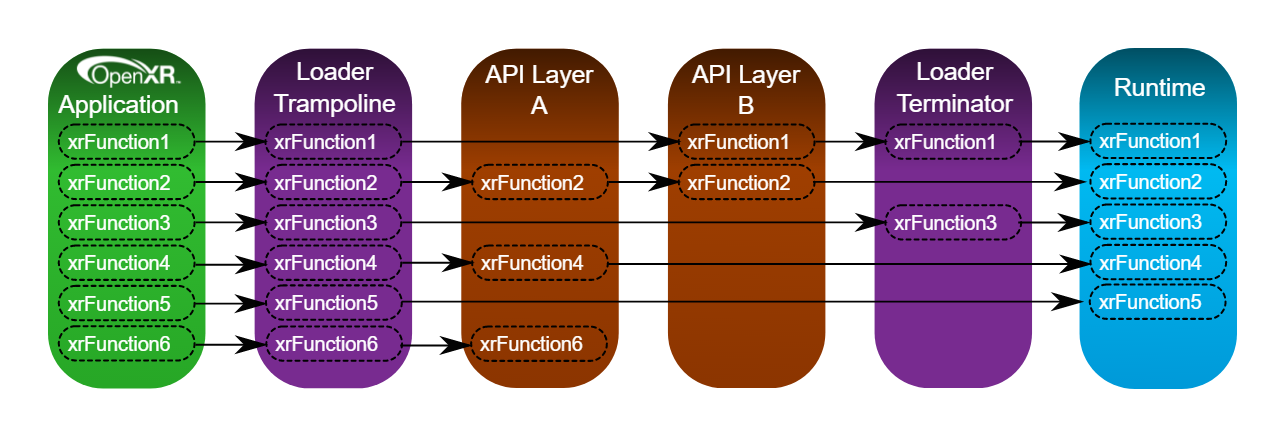
\includegraphics[width=1.0\textwidth]{imaxes/openxr_api_layer_graph.png}
  \caption{Explicación de la API por capas.}
  \label{fig:openxrapilayer}
\end{figure}

\subsection{OpenCV}
\acrfull{opencv} es una librería de código abierto que implementa principalmente funciones de visión artificial en tiempo real. Se utilizó para la generación y el seguimiento de los marcadores ARuco que forma parte de los paquetes adicionales de la librería.
\subsection{ARuco}
Los últimos años, los desarrollos de nuevos marcadores han tendido a un cuadrado negro con distintos patrones interiores \ref{fig:qrtags}, ya que permiten extraer la pose de la cámara a partir de sus 4 esquinas, asumiendo que esta esté adecuadamente calibrada \cite{GarridoJurado2014}. Esencialmente estos marcadores comparten ciertas características comunes en cuanto a su funcionamiento, entre todas las opciones disponibles se escogió ArUco como solución a nuestro proyecto por varios motivos:
\begin{itemize}
    \item Diccionarios generados dinámicamente.
    \item Posibilidad de crear tablas de marcadores lo que incrementa la resistencia a las oclusiones.
    \item Software para la calibración de cámara: De forma sencilla se puede calibrar cualquier cámara.
    \item La librería ha soportado el paso de los años sin problema, existiendo ejemplos y documentación extensa sobre el funcionamiento de la misma, facilitando así el desarrollo.
\end{itemize}


\begin{figure}[hp!]
  \centering
  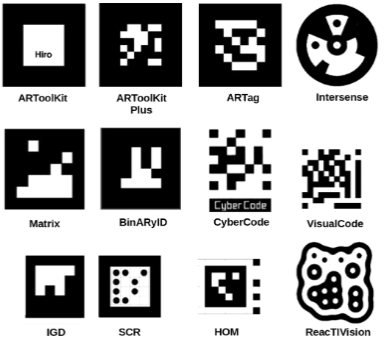
\includegraphics[width=0.75\textwidth]{imaxes/qrtags.png}
  \caption{Ejemplos de marcadores fiduciarios previos}
  \label{fig:qrtags}
\end{figure}

\subsection{Funcionamiento de Aruco}

\subsubsection*{Captura de imágenes o videos}
La captura de imágenes o vídeos se realiza mediante un dispositivo específico, como una cámara digital o un dispositivo móvil con cámara incorporada. En este paso se espera obtener una serie de imágenes o un vídeo sobre el que se espera encontrar uno o varios marcadores ARuco.
\subsubsection*{Conversión a escala de grises}
La conversión a escala de grises se realiza mediante el algoritmo de promedio ponderado de los canales RGB. Esta conversión reduce la cantidad de información a procesar y mejora la velocidad de procesamiento al trabajar con un único canal de información.
\subsubsection*{Aplicación de un filtro de bordes}
Para resaltar los bordes de los marcadores en la imagen se aplica un filtro de bordes. Un ejemplo común es el algoritmo de Canny, que se basa en la detección de gradientes y utiliza un umbral para determinar que bordes son relevantes y cuales no.
\subsubsection*{Detección de contornos}
Se utiliza un algoritmo de detección de contornos adaptativo para encontrar los contornos de los marcadores en la imagen. Un algoritmo común es el Transformada de Hough que permite detectar contornos circulares y lineales en la imagen. Este algoritmo busca patrones en la imagen que se correspondan con los contornos de los marcadores ARuco.
En un sistema de thresholding tradicional, se elige un umbral global para toda la imagen. Cualquier píxel con un valor de brillo superior al umbral se considera activo (p.ej. negro) y cualquier píxel con un valor de brillo inferior al umbral se considera inactivo (p.ej. blanco). Sin embargo, en muchas imágenes, el nivel óptimo de umbral puede variar entre diferentes partes de la imagen. El thresholding adaptativo se utiliza para solucionar este problema.

El thresholding adaptativo se divide en dos pasos:

Selección de una región de interés (ROI) en la imagen. Esta región puede ser de cualquier tamaño y forma.

Selección del umbral para cada pixel dentro de la ROI. El umbral se calcula a partir de la distribución de los niveles de gris dentro de la ROI.

Existen varios métodos para calcular el umbral adaptativo, algunos de los mas conocidos son:
\begin{itemize}
\item Método de media global
\item Método de la desviación estándar
\item Método de Otsu
\end{itemize}
Cada uno de estos métodos tiene sus propios pros y contras y en función de la aplicación y el tipo de imagen, se puede elegir uno u otro.
Además es posible modificar los siguientes parámetros para adecuar la librería a nuestro caso de uso, los más importantes son:
\begin{itemize}
    \item   \textbf{markerBorderBits:}
    El número de bits que se utilizan para representar el borde de un marcador. El borde de un marcador es el área blanca que rodea el patrón de código de barras en un marcador ARuco. El valor predeterminado es 4.
    \item \textbf{adaptiveThreshWinSizeMin and adaptiveThreshWinSizeMax:}
    El tamaño mínimo y máximo de la ventana utilizada para la umbralización adaptativa. La umbralización adaptativa es un método para determinar automáticamente el valor de umbral óptimo para una imagen. Estos parámetros se utilizan para especificar el tamaño de la ventana en píxeles que se utilizará para la umbralización adaptativa.
    \item \textbf{adaptiveThreshWinSizeMax:}
    Especificaa el paso o incremento con el cual se variará el tamaño de la ventana utilizada en la umbralización adaptativa.
    \item \textbf{adaptiveThreshConstant:}
    especificar una constante que se utilizará en el cálculo del valor de umbral para cada subregión de la imagen.
    \item \textbf{minMarkerPerimeterRate and maxMarkerPerimeterRate:}
    El porcentaje mínimo y máximo del perímetro de un marcador en relación con su área. Estos parámetros se utilizan para especificar el tamaño mínimo y máximo de los marcadores que se detectarán en la imagen.
    \item \textbf{minCornerDistanceRate:}
    La relación entre la distancia entre las esquinas de un marcador y su longitud de lado. Esto es utilizado para ignorar marcadores que tengan esquinas muy cercanas entre sí.
    \item \textbf{minDistanceToBorder:}
    La distancia mínima desde el borde de la imagen hasta el borde de un marcador. Esto se utiliza para ignorar marcadores que estén demasiado cerca del borde de la imagen.
    \item \textbf{ minMarkerDistanceRate:}
    La relación entre la distancia entre los marcadores y su longitud de lado. Esto se utiliza para ignorar marcadores que estén demasiado cerca entre sí.
\end{itemize}

\subsubsection*{Extracción de Bits}
Una vez que se han detectado los contornos de los posibles candidatos en una imagen, se analizan los bits extraídos de cada uno de estos para determinar si en efecto son marcadores o no.
Para ello se somete cada sección de la imagen a una corrección de perspectiva. A continuación se subdivide el candidato en la cantidad previamente establecida en el diccionario de bits que componen cada marcador. Dado que en un bit pueden encontrarse píxeles de los bits contiguos o errores en la imagen capturada por la cámara, se establece extrae el valor del bit en función de la desviación típica de los píxeles de dicho bit \ref{fig:mbe}.

\begin{figure}[hp!]
  \centering
  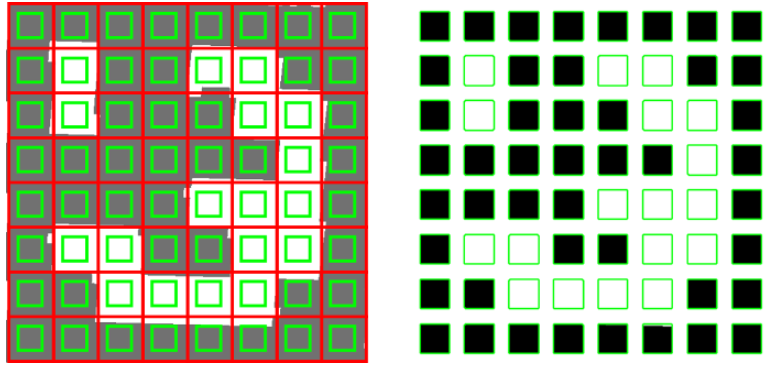
\includegraphics[width=0.85\textwidth]{imaxes/marker_bits_extraction.png}
  \caption{Proceso de extracción de Bits}
  \label{fig:mbe}
\end{figure}

\subsubsection*{Identificación de Marcadores}
Una vez determinados los bits de los que esta compuesto cada candidato a marcador es necesario determinar si el código extraído pertenece al diccionario y en caso de ser necesario aplicar algoritmos de corrección de errores.
La primera operación consiste en determinar la cantidad de bits erróneos permitidos en el borde de un marcador, ya que todos los marcadores ARuco cuentan al menos con un bit de borde. En lo que a corrección de errores se refiere, cada diccionario cuenta con un límite teórico de bits que pueden ser corregidos.

\subsubsection*{Refinado de Esquinas}
Una vez se han detectado e identificado todos los marcadores es posible realizar  un refinado a nivel de subpíxel de las esquinas para favorecer a la precisión del sistema. Este ultimo paso es altamente costoso a nivel computacional, pero se recomienda en aplicaciones en las que prima la precisión como es el caso.
\paragraph{}
Esta librería trabaja con un Pinhole Camera Model lo que quiere decir que se considera como el origen de coordenadas el punto en el que todos los rayos de lux convergerían en una supuesta cámara estenopeica ideal.

Las coordenadas se definen de la siquiente forma: Z crece frente a la camara mientras que X e Y se encuentran en el plano otrogonal de Z. X aumenta de derecha a izquierda e Y de abajo a arriba.




\begin{figure}[hp!]
  \centering
  
\includegraphics[width=0.3\textwidth]{imaxes/qr.png}
  \caption{Marcador Generado con ArUco}
  \label{fig:qr}
\end{figure}


\section{Hardware}
\subsection{Impresión 3D}
Se utilizaron dos impresoras 3D a lo largo del proyecto puesto que eran necesarios distintos requisitos para cada pieza.
Los modelos anatómicos debido a su complejidad se imprimieron en una impresora Fuse 1+ 30W que utiliza polvo de nylon para llevar a cabo las piezas.
Para los marcadores fiduciarios, se utilizo la Ultimaker 3, ya que se trata de figuras mas simples en las que la posibilidad de imprimir en distintos colores era especialmente importante.
\subsection{\acrfull{hmd}}
Para la implementación del sistema de captación de imagen y tracking se utilizó un casco HTC Vive Pro 2.


 \chapter{Metodología y Gestión del proyecto}
\label{chap:mygp}

 \chapter{Ejecución del proyecto}
\label{chap:edp}
Este capítulo tiene como objetivo tratar el desarrollo del proyecto en si mismo, así como discutir las opciones disponibles durante el progreso y las decisiones tomadas para llevarlo a cabo.
\section{Consideraciones previas}
Este trabajo nace como un desarrollo del proyecto troncal de \citeauthor{IglesiasGuitian2022} y como tal se debe ceñir a las condiciones que acarrea dicho proyecto.
Todo el equipo utilizado durante el desarrollo fue provisto por parte del mismo, o en su defecto por parte del \acrfull{citic}.
\section{Dificultades}
Dada la naturaleza del trabajo (altamente dependiente del hardware para su ejecución), es necesaria la presencialidad a lo largo de gran parte del desarrollo. Por causa mayor me he visto obligado a desplazarme al otro extremo de la península, lo que ha condicionado en parte el final del proyecto.
\section{Estudio inicial}
Se llevó a cabo un estudio para definir la hoja de ruta del proyecto. Dada la problemática a solventar, este trabajo alcanza a tocar áreas bien diferenciadas entre si que se pueden destacar como los pasos a seguir del mismo:
\begin{itemize}
    \item Extracción de volúmenes 3D a partir de un \acrshort{tc} válidos para su impresión.
    \item Diseñar un marcador fiduciario que permita el seguimiento de una pieza en 3 dimensiones y un método de acople al volumen previamente impreso.
    \item Implementar una solución que permita el seguimiento de dicho marcador.
    \item Integrar la solución sobre un \acrshort{hmd}.
\end{itemize}

Fruto de la investigación surge el artículo de  \citeauthor{MoretaMartinez2020} que expone una solución existente a los objetivos de este trabajo mediante el uso de software bajo licencia o de pago.  Es por ello que se toma una aproximación similar al problema sobre todo en las fases iniciales para la generación de los volúmenes, a pesar de afrontar de forma distintas las casuísticas finales.
\section{Generación de volúmenes a partir de TC}
Con el fin de facilitar la validación del progreso del proyecto, se utilizo una \acrshort{tc} de pruebas. Dichos datos contienen la sección superior (hombros y cabeza) de un sujeto \ref{fig:manix_full}. Durante el desarrollo se sugirió como posible caso práctico seleccionar el cráneo del sujeto en los datos de prueba y trabajar en la alineación 3D sobre el mismo, por lo que en las siguientes figuras se representa este objetivo.

\begin{figure}[hp!]
  \centering
  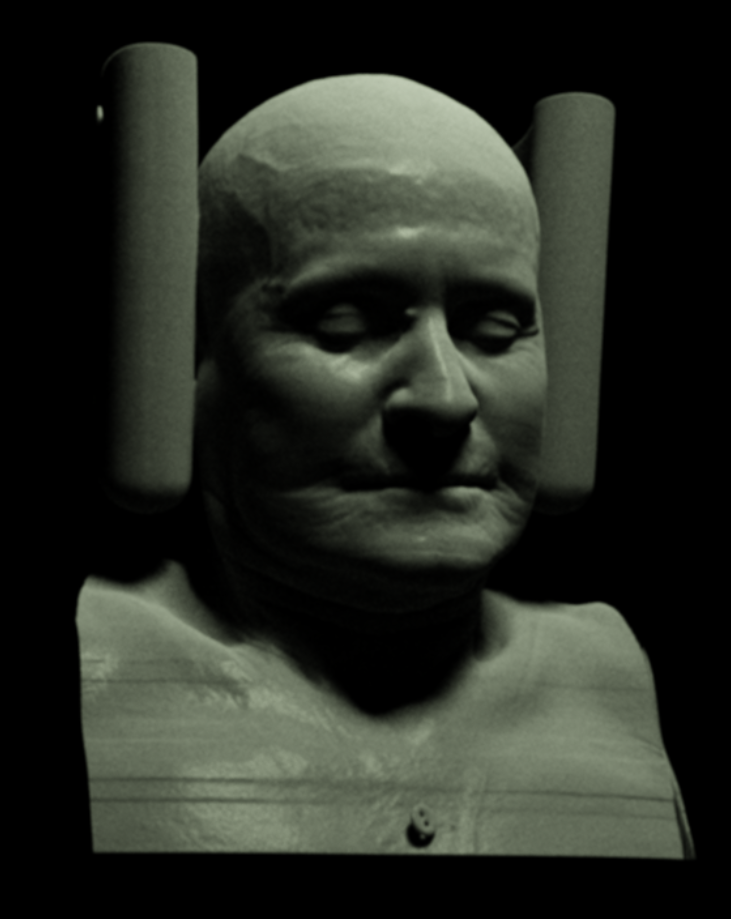
\includegraphics[width=0.75\textwidth]{imaxes/manix_full.png}
  \caption{Datos de prueba.}
  \label{fig:manix_full}
\end{figure}
Con el fin de seleccionar una sección concreta para exportar, se utilizaron las herramientas para segmentar volúmenes de Slicer3D
Nada mas abrir el programa se pueden ver las vistas, en las que se representará el \acrshort{tc} una vez se cargue \ref{fig:3dslier}.
Se utilizo principalmente la herramienta de "Thresholding" que permite seleccionar partes del modelo cuyas intensidades se comprenden en un intervalo o "threshold"  \ref{fig:seg_cr}. Posteriormente para eliminar las partes del modelo no deseadas se utilizo la herramienta de borrado hasta alcanzar el volumen deseado.

\begin{figure}%
    \centering
    \subfloat[\centering Captura de pantalla de 3DSlicer antes de cargar los datos.]{{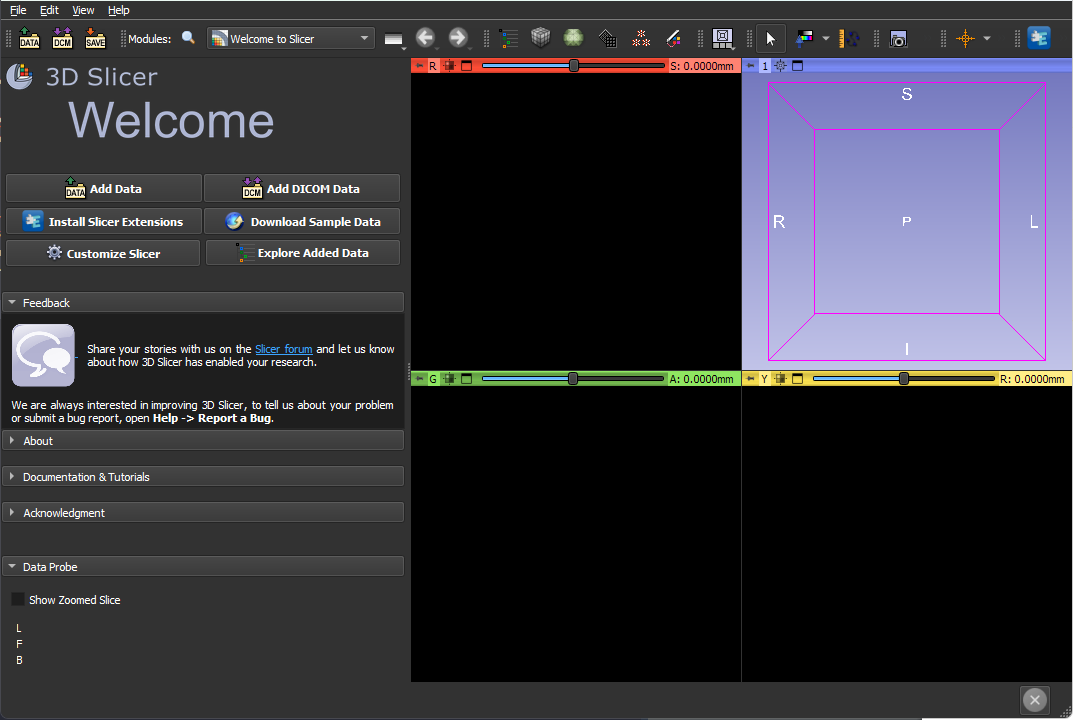
\includegraphics[width=6cm]{imaxes/captura3dslicer_1.png} }}%
    \qquad
    \subfloat[\centering  Captura de pantalla de 3DSlicer con los datos cargados.]{{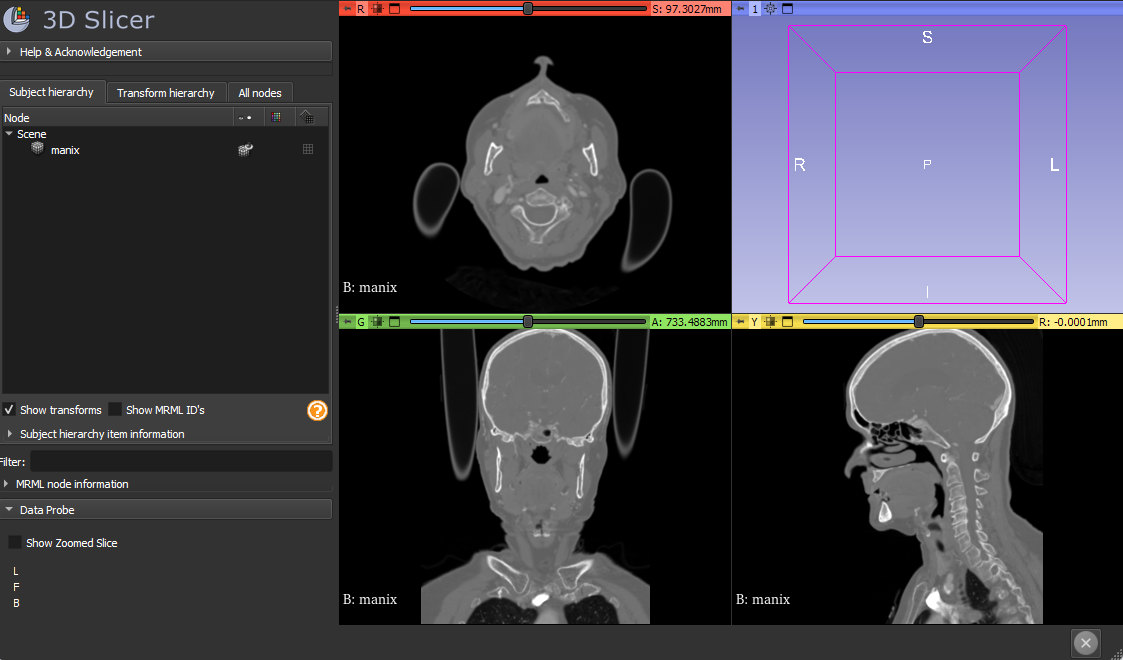
\includegraphics[width=6cm]{imaxes/captura3dslicer_2.png} }}%
    \caption{Capturas de 3DSlicer}%
    \label{fig:3dslier}%
\end{figure}


\begin{figure}[hp!]
  \centering
  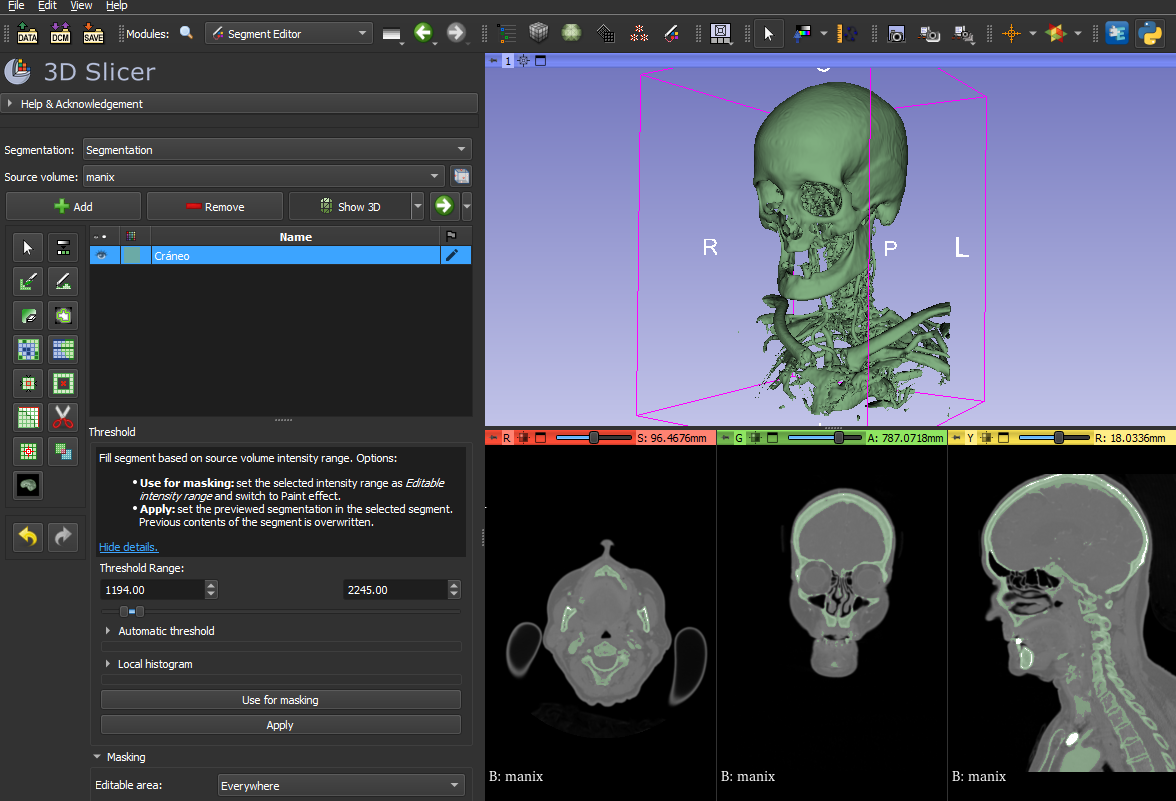
\includegraphics[width=0.75\textwidth]{imaxes/segment_craneo.png}
  \caption{Torso una vez aplicado el thresholding.}
  \label{fig:seg_cr}
\end{figure}
\section{Impresión 3D del volumen}
 Dado que el modelo no se genera a partir de figuras geométricas previas, es posible que presente geometrías rotas que a la hora del Slicing provocarán errores y no permitirán que se genere el GCODE correctamente.
 Por ello es necesario importar el modelo en un programa que nos facilite arreglar estas geometrías como es Meshmixer. En \ref{fig:arr_geo} se aprecia el modelo exportado, y cada marcador corresponde a errores producto de la exportación. Una vez reparados, se procede a imprimir la pieza.
 Como se comenta en \ref{chap:hs} para una pieza con una geometría tan compleja se requeriría una gran cantidad de soportes, por lo que se optó por la impresora Fuse 1 para la impresión de este modelo. A diferencia de una impresora 3D al uso, esta impresora utiliza un láser para fijar capa a capa el polvo de nylon, lo que garantiza una gran resolución en la pieza final y una gran durabilidad de la misma. Posterior al  trabajo de impresión es necesario retirar el material sobrante en la cámara de recuperación que cuenta con distintos utensilios para evitar malgastar el material sobrante ya que puede ser reutilizado.

\begin{figure}%
    \centering
    \subfloat[\centering Pieza en el proceso de recuperación del material.]{{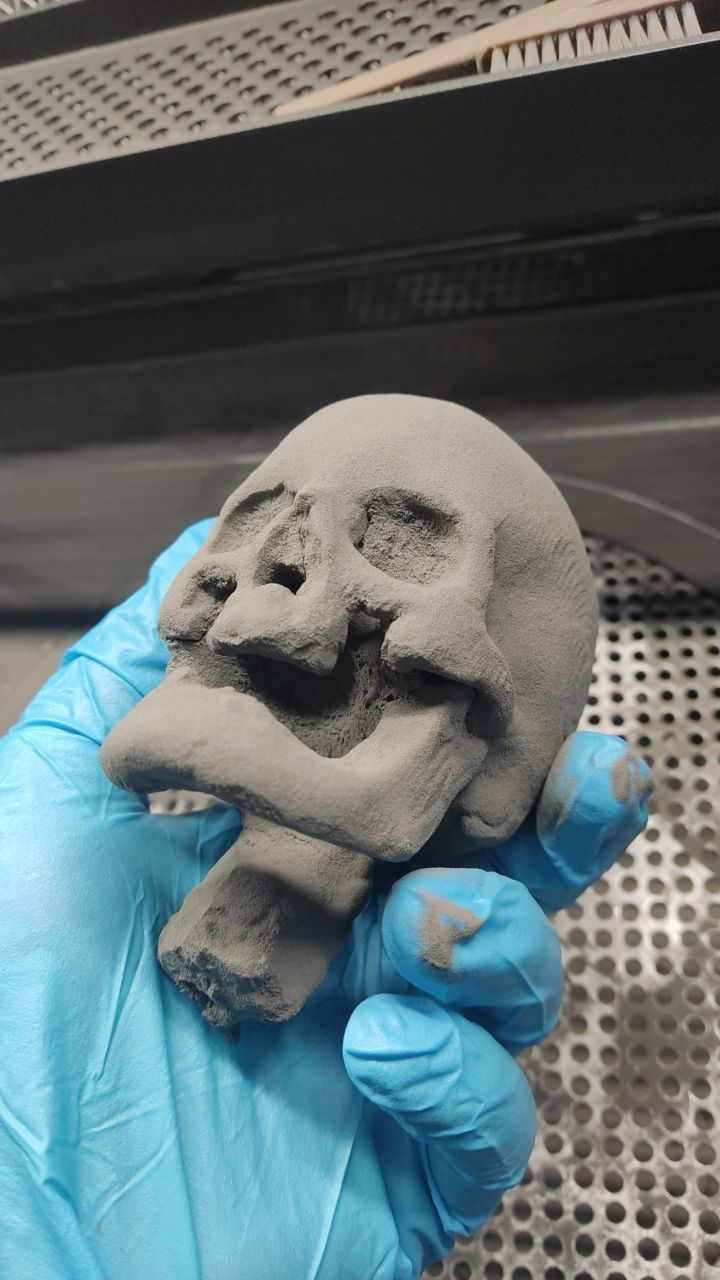
\includegraphics[width=6cm]{imaxes/limpiando_fig.png} }}%
    \qquad
    \subfloat[\centering  Pieza final.]{{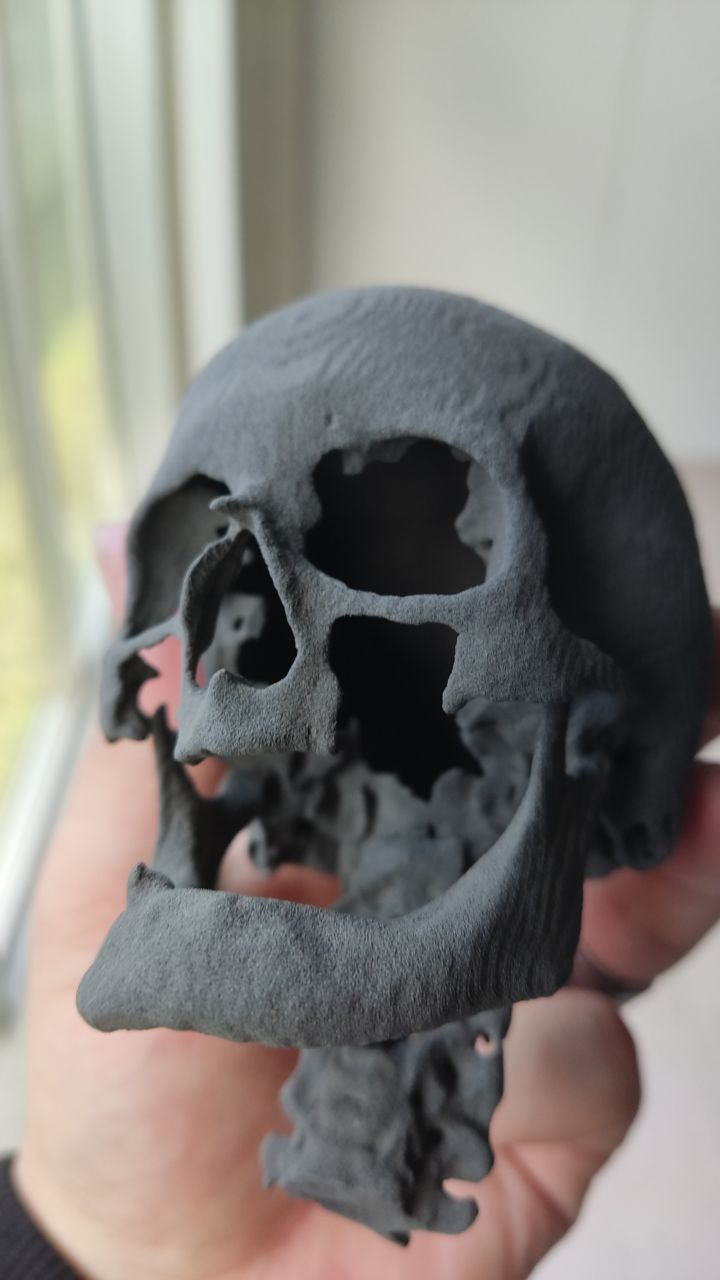
\includegraphics[width=6cm]{imaxes/limpia_fig.png} }}%
    \caption{Proceso de recuperación de material.}%
    \label{fig:3dslier}%
\end{figure}


\begin{figure}[hp!]
  \centering
  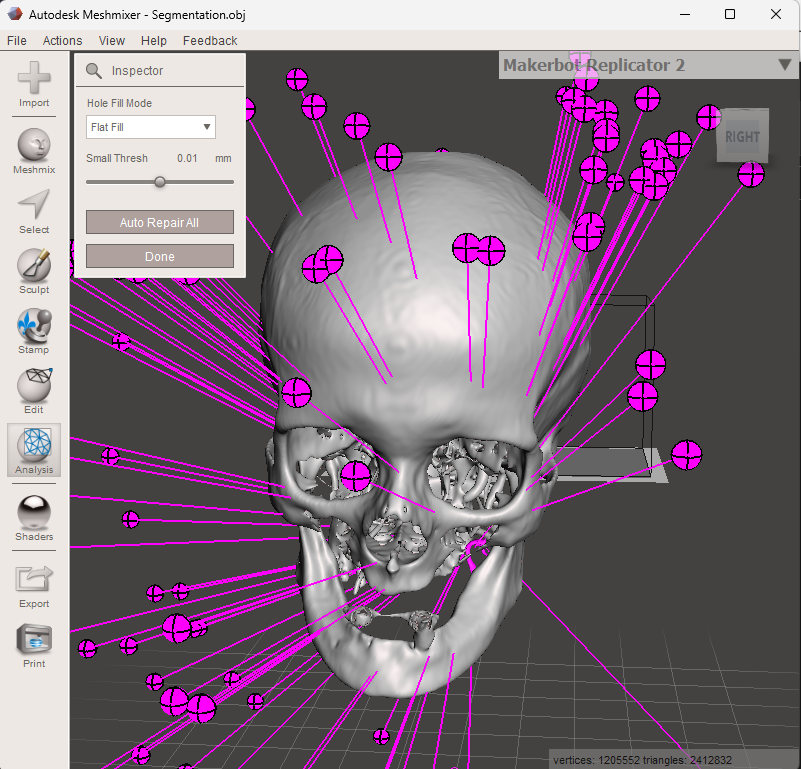
\includegraphics[width=0.75\textwidth]{imaxes/arreglo_geo.png}
  \caption{Modelo de cráneo 3D con geometrías erróneas.}
  \label{fig:arr_geo}
\end{figure}
 
\section{Desarrollo del marcador fiduciario}
Obtener la posición y rotación de una figura desconocida en el espacio es uno de los problemas principales a la hora de implementar soluciones de realidad virtual o aumentada, ya que requiere encontrar correspondencias entre objetos conocidos en el espacio y sus proyecciones en el vídeo.
Si bien existen aproximaciones que buscan puntos claves de las figuras o reconocen sus geometrías mediante técnicas de visión artificial e inteligencia artificial, se optó por el uso de  marcadores fiduciarios por varios motivos.
Primeramente, permite replicar el seguimiento del objeto independientemente del hardware utilizado, ya que una vez calibrada la cámara no se requiere ningún otro tipo de ajuste en el sistema. Otra ventaja es la robustez del sistema, ya que permite mantener el seguimiento a pesar de que parte del marcador se encuentre ocluido o no esté en el campo de visión de la cámara.
Dados los recursos disponibles, se optó por utilizar la librería ARuco para generar y seguir el marcador.
Debido a la versatilidad de las piezas con las que se pretende usar el marcador, se implementó priorizando eliminar las oclusiones del marcador por la pieza, por este motivo se diseñó como un cubo, de forma que al menos una cara sería visible en todo momento. A pesar de esto, utilizando un único marcador por cara cabe la posibilidad de que si parte del mismo se tapa, se pierda el seguimiento por completo dependiendo de que parte sea la afectada. Es por esto que se decidió implementar cada cara como una tabla de marcadores. Independientemente de la cara detectada el seguimiento se implementó de forma que se obtenga la rotación y posición del centro del cubo, transformando los valores obtenidos de cada cara para obtener este punto.

\paragraph{}
Se llevaron a cabo pruebas con distintos diccionarios de marcadores, modificando las tolerancias para los márgenes entre marcadores y los bordes del cubo con el fin de poder mantener unas dimensiones manejables sin comprometer el tamaño de cada marcador individual.
Finalmente fruto de los tests, se llegó al cubo \ref{fig:cubo_marker},
que cuenta con una matriz 2 x 2 de marcadores en cada cara.

\begin{figure}%
    \centering
    \subfloat[\centering Modelo del marcador fiduciario.]{{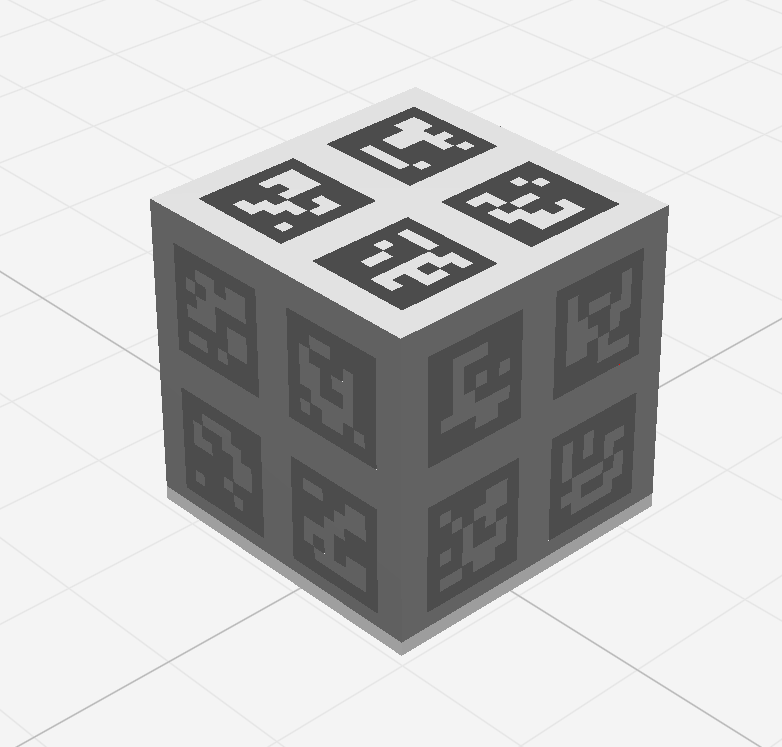
\includegraphics[width=6cm]{imaxes/cubo_marker.png} }}%
    \qquad
    \subfloat[\centering  Impresión del marcador fiduciario.]{{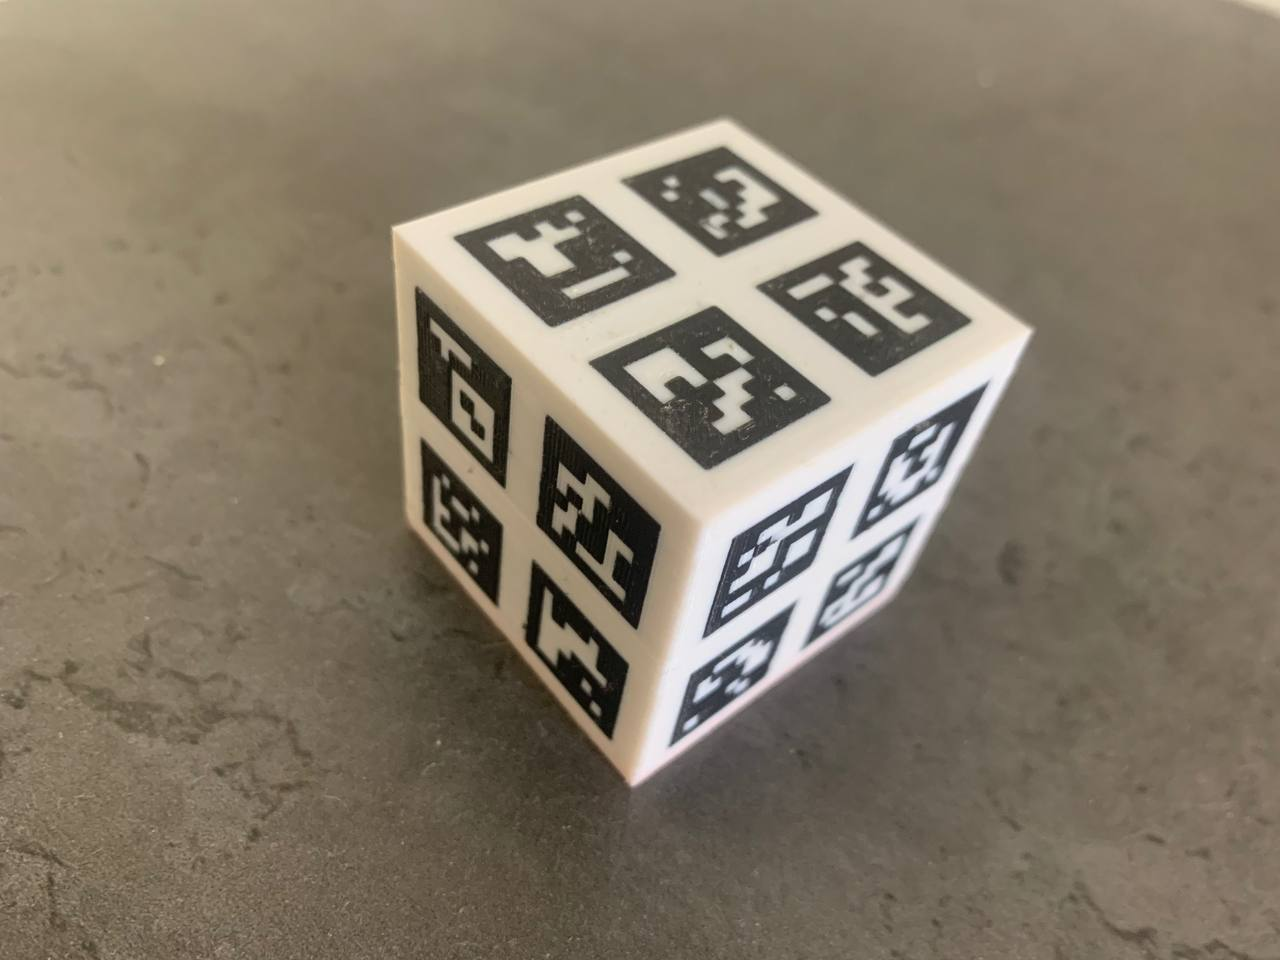
\includegraphics[width=6cm]{imaxes/cubo_marker_imp.png} }}%
    \caption{Diseño final del marcador fiduciario.}%
    \label{fig:3dslier}%
\end{figure}


\section{Implementación del Passthrough en Exposure Render}
Para la obtención de imágenes sobre las que poder trabajar se utilizaron las propias cámaras frontales del HTC Vive Pro 2. Se trata de un par de cámaras colocadas longitudinalmente a lo largo del frontal del casco, que permiten su uso en aplicaciones de realidad aumentada y realidad mixta. 
Para acceder a estas cámaras se debe hacer uso de SRworks C++ SDK. Este software en el momento del desarrollo del trabajo, en su versión nativa, presentaba errores que imposibilitaron la reconstrucción de la imagen para ser visualizada en el casco.
\section{Integración del software de tracking en Exposure Render}
Con el fin de analizar cada imagen con la mínima latencia posible, se implementaron dos threads individuales que esperan cada 16.6ms (ya que las cámaras tienen una tasa de refresco de 60Hz) para obtener una imagen de cada cámara. Dichas imágenes son analizadas para estimar la pose del marcador y modificar la posición del modelo con el que se esta trabajando en Exposure Render.
 \chapter{Conclusiones y trabajo futuro}
\label{chap:c}
\lettrine{C}{omo} cierre del trabajo, cabe reflexionar sobre el desarrollo del mismo así como sobre su estado actual, y su futuro. Dado por finalizado el trabajo, se han alcanzado buena parte de los objetivos fijados en su concepción:

\begin{itemize}
\item Se identificaron métodos para la extracción de secciones de \acrshort{tc} así como para el refinado de las mismas.También se analizaron las posibilidades de impresión optimizando el uso de los materiales y de las capacidades de las impresoras. Esto ha permitido trabajar sobre piezas en un nivel más visual e interactivo.
\item Se ha llevado a cabo un estudio de las soluciones existentes para el seguimiento 3D realizando pruebas de las mismas sobre los datos propios para extraer las ventajas y desventajas de cada solución en un nivel práctico.
\item Se han diseñado e impreso una gran cantidad de marcadores fiduciarios sobre los que se han realizado pruebas de forma iterativa con el fin de refinar y optimizar el diseño hasta obtener un resultado que satisface las características del proyecto. Todo esto mediante el uso de software libre creando así  un proceso adaptable a otros casos de uso.
\item Se ha integrado  la solución en el proyecto de \citeauthor{IglesiasGuitian2022} desvirtualizando un posible caso de uso. 
\end{itemize}
\subsection{Enriquecimiento Formativo}
Es imprescindible destacar la vertiente formativa que presenta este trabajo dada su naturaleza como trabajo de fin de grado. El autor ha tenido la posibilidad de trabajar sobre una serie de campos de los mas variados que comprenden la imagen médica, la impresión 3D, la visión artificial, la realidad virtual, el renderizado en un motor de trazado de rayos. Por otra parte, mencionar la exposición a un ambiente investigador en el \acrshort{citic} del que poder empaparse de la forma de trabajar y la cooperación entre iguales. También se trató de una primera puesta en práctica de los conceptos aprendidos sobre la gestión de proyectos que resultó enriquecedora.
\subsection{Trabajo futuro}
En la actualidad el proyecto tiene distintas vertientes que pueden ser desarrolladas en el futuro. Por una parte esta la mejora del sistema actual de seguimiento, si bien este en la actualidad es completamente funcional, en sistemas en los que la tasa de refresco de la cámara no es lo suficientemente alto el seguimiento puede dar una sensación de escalonado. Una posible solución sería aplicar algún tipo de filtrado de señales como puede ser un filtro de Kalman, que bien implementado, ayudaría a estimar pasos intermedios entre imágenes para proporcionar una experiencia mas confortable \cite{welch2020kalman}.
\paragraph{}
Una segunda vertiente de mejora, consistiría en reconstruír sobre las imágenes extraídas del casco, un ambiente de realidad aumentada, en el que se pudieran ver los modelos extraídos de las \acrshort{tc} sobre las mismas, donde aprovechándose de los desarrollos de la interfaz de realidad virtual del proyecto de \citeauthor{IglesiasGuitian2022} se pudiera trabajar con la pieza virtual modificando sus parámetros visuales.
\paragraph{}
Para terminar, otro posible desarrollo, consistiría en tratar de aumentar la resolución de las imágenes de las cámaras del casco, utilizando las imágenes de cada cámara para crear una imagen compuesta por ambas que permita una mejor detección del marcador fiduciario.
 %\chapter{Trabajo Futuro}
\label{chap:tf}

 %%%%%%%%%%%%%%%%%%%%%%%%%%%%%%%%%%%%%%%%
 % Apéndices, glosarios e bibliografía  %
 %%%%%%%%%%%%%%%%%%%%%%%%%%%%%%%%%%%%%%%%

 \appendix
 \appendixpage
 \chapter{Material adicional}
\label{chap:adicional}

\lettrine{E}{xemplo} de capítulo con formato de apéndice, onde se pode
incluír material adicional que non teña cabida no corpo principal do
documento, suxeito á limitación de 80 páxinas establecida no
regulamento de TFGs.

\Blindtext

%\include{anexos/...}

 \printglossary[type=\acronymtype,title=\nomeglosarioacronimos]
 \printglossary[title=\nomeglosariotermos]

 \bibliographystyle{IEEEtranN}
 \bibliography{\bibconfig,bibliografia/bibliografia}
 \clearpage
 
\end{document}

%%%%%%%%%%%%%%%%%%%%%%%%%%%%%%%%%%%%%%%%%%%%%%%%%%%%%%%%%%%%%%%%%%%%%%%%%%%%%%%%
